%% LyX 2.4.4 created this file.  For more info, see https://www.lyx.org/.
%% Do not edit unless you really know what you are doing.
\documentclass[english]{article}
\usepackage[T1]{fontenc}
\usepackage[latin9]{inputenc}
\usepackage{units}
\usepackage{enumitem}
\usepackage{amsmath}
\usepackage{amsthm}
\usepackage{geometry}
\geometry{verbose,tmargin=1in,bmargin=1in,lmargin=1in,rmargin=1in}
\PassOptionsToPackage{normalem}{ulem}
\usepackage{ulem}

\makeatletter
%%%%%%%%%%%%%%%%%%%%%%%%%%%%%% Textclass specific LaTeX commands.
\numberwithin{equation}{section}
\numberwithin{figure}{section}
\newlength{\lyxlabelwidth}      % auxiliary length 

%%%%%%%%%%%%%%%%%%%%%%%%%%%%%% User specified LaTeX commands.
\usepackage{fancyhdr}
\usepackage{lastpage}
\pagestyle{fancy}
\usepackage{enumitem}
\usepackage{ifthen}
\everymath=\expandafter{\the\everymath\displaystyle}
%\DeclareMathSizes{10}{10}{10}{10}
\usepackage{multicol}

\usepackage{tikz}
\usepackage{tikz-3dplot}
\usetikzlibrary{calc,arrows}

\usetikzlibrary{patterns}
\usetikzlibrary{plotmarks}
\usepackage{pgfplots}
\pgfplotsset{compat=newest}
\usepgfplotslibrary{polar}

\usepackage{calc}
\usepackage[nomessages]{fp}

\usepackage{datetime}
% Added by lyx2lyx
\setlength{\parskip}{\smallskipamount}
\setlength{\parindent}{0pt}

\makeatother

\usepackage{babel}
\begin{document}
\renewcommand{\author}{Dr.\,James Ashe}

\newcommand{\classNum}{331}

\newcommand{\classSec}{A}

\newcommand{\nameType}{Name:}

\newcommand{\examType}{Final Exam}

\renewcommand{\date}{\formatdate{3}{12}{2013}} %%\today

%%First page's header%%%%%%%%%%%%%%%%%%%%%%
\fancypagestyle{firststyle} %%header settings for first pagr
{
	\fancyhead[L]{MTH \classNum{}(\classSec{}) \author{}\\
	\textbf{\examType{}} \date{}}
	\fancyhead[C]{\textbf{\nameType}}
	\setlength{\headsep}{14pt}
}
%%%%%%%%%%%%%%%%%%%%%%%%%%%%%%%%%%%%%%%%%%

%%Next page's header%%%%%%%%%%%%%%%%%%%%%%%
\setlist{nolistsep}
\lhead{MTH \classNum{}(\classSec{})} 
\chead{\textbf{\nameType}} 
\cfoot{\thepage{}~of~\pageref{LastPage}} 
\setlength{\headsep}{5pt} 
%%%%%%%%%%%%%%%%%%%%%%%%%%%%%%%%%%%%%%%%%%%

%%Various settings; see the preamble for other settings%%%%%
%%\setenumerate[0]{leftmargin=12pt,itemindent=0pt,labelwidth=0pt}
\renewcommand{\labelenumi}{\textbf{\arabic{enumi}.}}
\renewcommand{\labelenumii}{\textbf{\alph{enumii}.}}
\thispagestyle{firststyle}

\newcommand{\xspace}{\vspace{0cm}}
\newcounter{probs}
%%%%%%%%%%%%%%%%%%%%%%%%%%%%%%%%%%%%%%%%%%

\textbf{Show your work. All problems are worth 4 point unless stated
otherwise.}
\begin{enumerate}[resume]
\item Write the expression, $x+x^{2}+x^{3}+x^{4}+\cdots+x^{20}$ in sigma
notation.

\begin{enumerate}[resume]
\item []${\displaystyle \sum_{n=1}^{20}x^{n}}$\vfill\addtocounter{probs}{1}
\end{enumerate}
\item Write out the following sum ${\displaystyle \sum_{n=0}^{3}n^{2}}$.

\begin{enumerate}[resume]
\item []${\displaystyle \sum_{n=0}^{3}n^{2}}=0+1^{2}+2^{2}+3^{2}=1+4+9=14$\vfill\addtocounter{probs}{1}
\end{enumerate}
\end{enumerate}
\emph{Evaluate the geometric series or state that it diverges. }
\begin{enumerate}[resume]
\item ${\displaystyle \sum_{k=0}^{\infty}\frac{1}{4^{k}}}$

\begin{enumerate}[resume]
\item []${\displaystyle {\displaystyle \sum_{k=0}^{\infty}\frac{1}{4^{k}}=\sum_{k=0}^{\infty}1\left(\frac{1}{4}\right)^{k}}}=\frac{1}{1-\nicefrac{1}{4}}=\frac{4}{3}$
since $r=\nicefrac{1}{4}<1$. \vfill\addtocounter{probs}{1}
\end{enumerate}
\item ${\displaystyle \sum_{m=0}^{\infty}\frac{(-3)^{2n}}{5^{n}}}$

\begin{enumerate}[resume]
\item []${\displaystyle \sum_{m=0}^{\infty}\frac{(-3)^{2n}}{5^{n}}={\displaystyle \sum_{m=0}^{\infty}\left(\frac{9}{5}\right)^{n}}=\infty}$
since $r=\nicefrac{9}{5}>1$\vfill\addtocounter{probs}{1}
\end{enumerate}
\end{enumerate}
\emph{Using the Squeeze Theorem, find the limit of the following sequence
or determine that the limit does not exist.}
\begin{enumerate}[resume]
\item ${\displaystyle \lim_{n\rightarrow\infty}\left\{ \frac{(-1)^{n}}{n}\right\} }$

\begin{enumerate}[resume]
\item []$\frac{-1^{n}}{n}\leq\frac{(-1)^{n}}{n}\leq\frac{1^{n}}{n}$ and
${\displaystyle \lim_{n\rightarrow\infty}\left\{ \frac{-1^{n}}{n}\right\} ={\displaystyle \lim_{n\rightarrow\infty}\left\{ \frac{1^{n}}{n}\right\} =0}}$
so by the Squeeze Theorem, ${\displaystyle \lim_{n\rightarrow\infty}\left\{ \frac{(-1)^{n}}{n}\right\} =0}$.\vfill\addtocounter{probs}{1}
\end{enumerate}
\end{enumerate}
\emph{Use the Divergence Test to determine whether the following series
diverge, or state that the test is inconclusive.}
\begin{enumerate}[resume]
\item ${\displaystyle \sum_{k=0}^{\infty}\frac{1}{k+1}}$

\begin{enumerate}[resume]
\item []${\displaystyle \lim_{n\rightarrow\infty}\frac{1}{n+1}=0}$, so
then the test is inconclusive.\vfill\addtocounter{probs}{1}
\end{enumerate}
\end{enumerate}
\newpage
\begin{enumerate}[resume]
\item Let $f(x)=3e^{x}$. (Each part is worth 4 points.)

\begin{enumerate}[resume]
\item Find the Taylor polynomial of order $n=2$ for $f(x)$ centered at
$0$.

\begin{enumerate}[resume]
\item []$f'(x)=3e^{x}$ and $f''(x)=3e^{x}$. So then 
\begin{eqnarray*}
p_{2}(x) & = & f(0)+f'(0)(x)+\frac{f''(0)}{2}(x)^{2}\\
 & = & 3+3x+\frac{3}{2}x^{2}
\end{eqnarray*}
\vfill\addtocounter{probs}{1}
\end{enumerate}
\item Use the Taylor polynomial from above to approximate $3e^{0.1}$, and
compute the absolute error in the approximation assuming the exact
value is given by a calculator.

\begin{enumerate}[resume]
\item []$p_{2}(.1)=3+3(.1)+\frac{3}{2}(.1)^{2}=3.315$ and $3e^{0.1}\approx3.31551$.
So $\left|3e^{0.1}-3.315\right|\approx.000513$\vfill\addtocounter{probs}{1}
\end{enumerate}
\end{enumerate}
\end{enumerate}
\emph{Give a set of parametric equations that describes the curve.}
\begin{enumerate}[resume]
\item Give two different sets of parametric equations that generate a circle
centered at $(0,0)$ with radius $5$.

\begin{enumerate}[resume]
\item {[}2 pts{]} Set one:

\begin{enumerate}[resume]
\item []There are many answers: $x=5\cos t$ and $y=5\sin t$\vspace{1cm}\addtocounter{probs}{1}
\end{enumerate}
\item {[}2 pts{]} Set two:

\begin{enumerate}[resume]
\item []There are many answers: $x=5\cos(-t)$ and $y=5\sin(-t)$\vspace{1cm}\addtocounter{probs}{1}
\end{enumerate}
\end{enumerate}
\end{enumerate}
\emph{Locate the following polar coordinates on a graph. }
\begin{enumerate}[resume]
\item A:$\left(1.5,\frac{\pi}{6}\right)$, B:$\left(1.5,\frac{\pi}{6}+\frac{\pi}{2}\right)$,
C:$\left(1.5,-\frac{\pi}{6}\right)$, D:$\left(-1.5,-\frac{\pi}{6}\right)$

\begin{enumerate}[resume]
\item []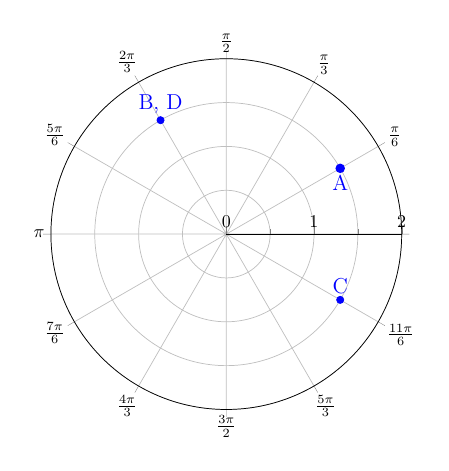
\begin{tikzpicture} [scale=.65] 
	\begin{polaraxis}[
			xmin=0,xmax=360,
			ymin=0,ymax=2,
			ytick={0,1,...,20}, 
			%minor x tick num={4},
			minor y tick num={1},
			grid=both,
			%yticklabels={,,,1,,,2,,}, 
			xticklabels={,,$\frac{\pi}{6}$,$\frac{\pi}{3}$,$\frac{\pi}{2}$,$\frac{2\pi}{3}$,$\frac{5\pi}{6}$,$\pi$,$\frac{7\pi}{6}$,$\frac{4\pi}{3}$,$\frac{3\pi}{2}$,$\frac{5\pi}{3}$,$\frac{11\pi}{6}$,}
		]
		%\addplot+[black, very thick, mark=none, domain=0:720, samples=600 ] {2-5*cos(x)};
		%\addplot+[gray, very thin, mark=none, domain=0:720, samples=600 ] {1.5};
		%\addplot+[black, mark = *, nodes near coords=mylabel,every node near coord/.style={anchor=180}] coordinates ( 30: 1.5);
		%\draw (30:1.5) circle[radius=2pt];
		\addplot[color=blue,solid,mark=*,very thick] coordinates {(30,1.5)} node[below] {\large{A}};
		\addplot[color=blue,solid,mark=*] coordinates {(120,1.5)} node[above] {\large{B, D}};
	\addplot[color=blue,solid,mark=*] coordinates {(-30,1.5)} node[above] {\large{C}};
	\end{polaraxis}
	%\draw (3.43cm,-.7cm) node [below] {$r=2-5\cos\theta $}; 
\end{tikzpicture}\addtocounter{probs}{1}
\end{enumerate}
\end{enumerate}
\newpage

\emph{Express the following }\textbf{\emph{polar}}\emph{ coordinates
in }\textbf{\emph{Cartesian}}\emph{ coordinates.}
\begin{enumerate}[resume]
\item $\left(2,\frac{\pi}{3}\right)$

\begin{enumerate}[resume]
\item []$x=2\cos\nicefrac{\pi}{3}=1$ and $y=2\sin\nicefrac{\pi}{3}=\sqrt{3}$\\
coordinates: $(1,\sqrt{3})$\vfill\addtocounter{probs}{1}
\end{enumerate}
\end{enumerate}
\emph{Use the graph to draw the following vectors (provide labels).
Make certain to indicate direction.}
\begin{enumerate}[resume]
\item \begin{multicols}{2}

\begin{enumerate}[resume]
\item {[}2 pts{]}\textbf{ $\frac{1}{2}\mathbf{v}$}
\item {[}2 pts{]} $\mathbf{u}+\mathbf{v}$ 
\end{enumerate}
\columnbreak\tdplotsetmaincoords{0}{0}% %%specifes orientation %%\tdplotsetrotatedcoords{0}{20}{0}% %%specifes angle of rotation
\begin{tikzpicture} 		
	[tdplot_main_coords,
		scale=.5,
		grid/.style={very thin,gray}, 
		axis/.style={->,black,thick},
		vector/.style={very thick,red,-stealth},
		vector guide/.style={dashed,red,thick},
		angle/.style={black,thick}]
	
	%draw a grid in the x-y plane 	
	%\foreach \x in {-1,0,...,1} 		
	%\foreach \y in {-1,0,...,1} 		
	{ 			
		%\draw[grid] (\x,-0.25) -- (\x,1.25); 			
		%\draw[grid] (-0.25,\y) -- (1.25,\y); 		
	} 		
	
	%draw the axes 	
	\draw[axis] (-2.5,0) -- (4.5,0) node[anchor=west]{$x$}; 	
	\draw[axis] (0,-1) -- (0,5) node[anchor=west]{$y$}; 	

	%standard tikz coordinate definition using x, y, z coords 	
	\coordinate (O) at (0,0);

	%draw vectors
	\draw[->, very thick,red,-stealth] (0,0) -- (4,2) node[anchor=south west]{\textbf{u}} node[anchor=north east,pos=.6]{$$};
	\draw[->,very thick,blue,-stealth] (0,0) -- (-2,3) node[anchor=south west]{\textbf{v}} node[anchor=north east,pos=.6]{$$};
	\draw[very thick,black,-stealth] (0,0) -- (2,1) node[anchor=south east]{(a)} node[anchor=north east,pos=.6]{$$};
	\draw[very thick,black,-stealth] (0,0) -- (2,5) node[anchor=south west]{(b)} node[anchor=north east,pos=.6]{$$};
	\draw[dashed,black] (-2,3) -- (2,5) node[anchor=south west]{} node[anchor=north east,pos=.6]{$$};
	\draw[dashed,black] (2,5) -- (4,2) node[anchor=south west]{} node[anchor=north east,pos=.6]{$$};
	%\draw[very thick,black,-stealth] (3,1) -- (4,4) node[anchor=south east]{(c)} node[anchor=north east,pos=.6]{$$};
	%\draw[black] (0,0) -- (0,0) node[anchor=south west]{$\theta$};
	%draw an arc illustrating the angle defining the orientation 
	%\tdplotsetthetaplanecoords{45}	
	%\tdplotdrawarc[tdplot_rotated_coords,angle]{(O)}{.35}{54.7}{90}{anchor=west}{$\phi$} %{center}{radius}{start}{end angle}
\end{tikzpicture}
	\end{multicols}\addtocounter{probs}{1}
\end{enumerate}
\emph{Use the vectors $\mathbf{u}=\left\langle -1,1,1\right\rangle $
and $\mathbf{v}=\left\langle 2,-4,0\right\rangle $ to complete the
following problems.}
\begin{enumerate}[resume]
\item $\mathbf{u\cdot}\mathbf{v}$

\begin{enumerate}[resume]
\item []$\left\langle -1,1,1\right\rangle \cdot\left\langle 2,-4,0\right\rangle =-1(2)+1(-4)+1(0)=-2-4=-6$\vfill\addtocounter{probs}{1}
\end{enumerate}
\item Find the angle between $\mathbf{u}$ and $\mathbf{v}$. ($|\mathbf{u}|=\sqrt{3}$
and $|\mathbf{v}|=2\sqrt{5}$.) 

\begin{enumerate}[resume]
\item []$\mathbf{u\cdot}\mathbf{v}=-6=\sqrt{3}2\sqrt{5}\cos\theta\Rightarrow\theta=\cos^{-1}\left(-\frac{3}{\sqrt{15}}\right)\approx2.457$\vfill\addtocounter{probs}{1}
\end{enumerate}
\item Find a vector perpendicular to $\mathbf{u}$ and $\mathbf{v}$.

\begin{enumerate}[resume]
\item [](answers may vary) $\mathbf{u}\times\mathbf{v}=\det\begin{vmatrix}\begin{array}{rrr}
\mathbf{i} & \mathbf{j} & \mathbf{k}\\
-1 & 1 & 1\\
2 & -4 & 0
\end{array}\end{vmatrix}=4\mathbf{i}+2\mathbf{j}+2\mathbf{k}$\\
$\mathbf{n}=\left\langle 4,2,2\right\rangle $\vfill\addtocounter{probs}{1}
\end{enumerate}
\end{enumerate}
\newpage
\begin{enumerate}[resume]
\item A woman paddles a canoe at 5 mi/hr at 30 degrees ($\frac{1}{6}\pi$
radians) north of east. Find a vector describing the vertical and
horizontal components of the canoe's velocity.

\begin{enumerate}[resume]
\item []$\left\langle 5\cos\left(\nicefrac{\pi}{6}\right),5\sin\left(\nicefrac{\pi}{6}\right)\right\rangle =\left\langle \nicefrac{5\sqrt{3}}{2},\nicefrac{5}{2}\right\rangle $\vfill\addtocounter{probs}{1}
\end{enumerate}
\end{enumerate}
\emph{Find the indicated partial derivative of the following functions.}
\begin{enumerate}[resume]
\item Find $f_{x}$ and $f_{y}$ for $f(x,y)=5x\cdot\sin2xy$.

\begin{enumerate}[resume]
\item []$f_{x}=5\sin2xy+10xy\cdot\cos2xy$
\item []$f_{y}=10x^{2}\cos2xy$\vfill\addtocounter{probs}{1}
\end{enumerate}
\item Find the four second partial derivatives of $f(x,y)=2x^{5}y^{2}+2x^{2}$.

\begin{enumerate}[resume]
\item []$f_{x}=10x^{4}y^{2}+4x$ and $f_{y}=4x^{5}y^{2}$, so
\item []$f_{xx}=40x^{3}y^{2}+4$, $f_{yy}=8x^{5}y$, and $f_{xy}=f_{yx}=20x^{4}y$\vfill\addtocounter{probs}{1}
\end{enumerate}
\end{enumerate}
\emph{Use the Chain Rule to find the following derivative. When feasible
express your answer in terms of the independent variable. }
\begin{enumerate}[resume]
\item $dW/dt$ where $W=x^{2}+y^{2}$, $x=\cos2t$, and $y=\sin2t$.

\begin{enumerate}[resume]
\item []$\frac{dW}{dt}=\frac{dw}{dx}\frac{dx}{dt}+\frac{dw}{dy}\frac{dy}{dt}=(2x)(-2\sin2t)+(2y)(2\cos2t)=(2\cos2t)(-2\sin2t)+(2\sin2t)(2\cos2t)=0$\vfill\addtocounter{probs}{1}
\end{enumerate}
\end{enumerate}
\newpage

\emph{Compute the gradient of the following function and evaluate
it at the given point P.}
\begin{enumerate}[resume]
\item $f(x,y)=e^{2xy}$; $P(2,3)$

\begin{enumerate}[resume]
\item []$f_{x}=2ye^{2xy}$ and $f_{y}=2xe^{2xy}$, so $\nabla f(2,3)=\left\langle 2ye^{2xy},2xe^{2xy}\right\rangle |_{\left(2,3\right)}=\left\langle 4e^{12},6e^{12}\right\rangle $\vfill\addtocounter{probs}{1}
\end{enumerate}
\end{enumerate}
\emph{Let $f(x,y)=\ln(xy)$ and $P(2,3)$ be a point on $f$. }
\begin{enumerate}[resume]
\item Find a vector that points in a direction of steepest ascent in $f$
at $P$.

\begin{enumerate}[resume]
\item []Any vector in the direction of: $\nabla f(2,3)=\left\langle \frac{1}{x},\frac{1}{y}\right\rangle |_{(2,3)}=\left\langle \frac{1}{2},\frac{1}{3}\right\rangle $\vfill\addtocounter{probs}{1}
\end{enumerate}
\item Find a vector that points in a direction of no change in $f$ at $P$.

\begin{enumerate}[resume]
\item []Any vector parallel to: $\left\langle -\frac{1}{3},\frac{1}{2}\right\rangle $\vfill\addtocounter{probs}{1}
\end{enumerate}
\end{enumerate}
\emph{Use the Second Derivative Test to determine (if possible) whether
each critical point of the given function is a local maximum, local
minimum, saddle point, or inconclusive.}
\begin{enumerate}[resume]
\item {[}8 pts{]} $g(x,y)=x^{4}+y^{4}-16xy$ with critical points $(0,0)$,
$(2,2)$, and $(-2,-2)$.

\begin{enumerate}[resume]
\item [$(0,0)$:]$D_{g}=g_{xx}g_{yy}-g_{xy}^{2}=(12x^{2})(12y^{2})-(-16)^{2}=144x^{2}y^{2}$\\
$D_{g}(0,0)=-16^{2}<0$ so $f$ has a \uline{saddle point} at $(0,0)$
\item [$(2,2)$:]$D_{g}(2,2)=12^{2}16-16^{2}>0$ and $g_{xx}(2,2)=12(4)>0$
so $g(2,2)$ is a \uline{local minimum}.
\item [$(-2,-2)$:]$D_{g}(-2,-2)=12^{2}16-16^{2}>0$ and $g_{xx}(-2,-2)=12(4)>0$
so $g(-2,-2)$ is a \uline{local minimum}.\vfill\xspace\xspace\addtocounter{probs}{1}\addtocounter{probs}{1}%\arabic{probs}
\end{enumerate}
\end{enumerate}

\subsubsection*{BONUS}

\emph{Use Lagrange multipliers to find the maximum and minimum values
of $f$ (when they exist) subject to the constraint.}
\begin{enumerate}[resume]
\item $f(x,y)=e^{2xy}$ subject to $x^{3}+y^{3}=16$
\item 
\end{enumerate}

\end{document}
